\begin{frame}[c]
	\tableofcontents[currentsection, hideothersubsections]
\end{frame}

\subsection{Cahier des charges}
\begin{frame}[c]
	\frametitle{Cahier des Charges}
	\begin{block}{Besoins}
		\begin{description}
			\item[Client :] s'enregistrer, jouer, demander l'état du jeu, se désinscrire
			\item[Serveur :] envoyer un message à tous les utilisateurs
		\end{description}
	\end{block}
	\begin{block}{Contraintes}
		\begin{itemize}
			\item Réaliser une application distribuée avec un nombre illimité (?) de clients
			\item Clients de tous types : Linux, Android, iOS, Windows, Mac\dots{}
			\item Le jeu se déroule en temps réel et les actions d'un client influencent les autres clients
		\end{itemize}
	\end{block}
\end{frame}

\subsection{Technologies étudiées}
\begin{frame}[c]
	\frametitle{Technologies étudiées}
	\begin{block}{6 possibilités envisagées}
		\begin{itemize}
			\item Sockets
			\item RMI
			\item Corba
			\item WebServices
			\item EJB
			\item REST
		\end{itemize}
	\end{block}
\end{frame}

\begin{frame}[c]
	\frametitle{Sockets}
	\begin{block}{Avantages}
		\begin{itemize}
			\item Implémentation du minimum nécessaire : gain de rapidité
			\item Très bas niveau donc portable
		\end{itemize}
	\end{block}
	\begin{block}{Inconvénient}
		\begin{itemize}
			\item Difficulté de mise en place
		\end{itemize}
	\end{block}
\end{frame}

\begin{frame}[c]
	\frametitle{RMI}
	\begin{block}{Avantages}
		\begin{itemize}
			\item Callbacks inclus dans la technologie 
			\item Les objets sont situés côté serveur : gain de performance côté client
		\end{itemize}
	\end{block}
	\begin{block}{Inconvénient}
		\begin{itemize}
			\item Pas de librairie Android
		\end{itemize}
	\end{block}
\end{frame}

\begin{frame}[c]
	\frametitle{Corba}
	\begin{block}{Avantages}
		\begin{itemize}
			\item Callbacks inclus dans la technologie 
			\item Les objets sont situés côté serveur : gain de performance côté client
		\end{itemize}
	\end{block}
	\begin{block}{Inconvénients}
		\begin{itemize}
			\item Pas de librairie Android
			\item Difficulté de mise en place
		\end{itemize}
	\end{block}
\end{frame}

\begin{frame}[c]
	\frametitle{WebServices}
	\begin{block}{Avantages}
		\begin{itemize}
			\item Portabilité
			\item Simplicité de mise en place
		\end{itemize}
	\end{block}
	\begin{block}{Inconvénients}
		\begin{itemize}
			\item Callbacks absents sans un serveur (ex : JBOSS)
		\end{itemize}
	\end{block}
\end{frame}

\begin{frame}[c]
	\frametitle{EJB}
	\begin{block}{Avantages}
		\begin{itemize}
			\item Callbacks inclus dans la technologie 
		\end{itemize}
	\end{block}
	\begin{block}{Inconvénient}
		\begin{itemize}
			\item Pas de librairie Android
		\end{itemize}
	\end{block}
\end{frame}

\begin{frame}[c]
	\frametitle{REST}
	\begin{block}{Avantages}
		\begin{itemize}
			\item Architecture de haut niveau : simplicité d’implémentation
			\item Leger
			\item Framework complet dans Android et Java
			\item Framework compatible pour iOS (ASIHTTPRequest)
		\end{itemize}
	\end{block}
	\begin{block}{Inconvénients}
		\begin{itemize}
			\item Aucune connaissance préalable sur la vitesse de transfert
			\item Pas de callbacks
		\end{itemize}
	\end{block}
	\begin{center}
		$\Rightarrow$ notre choix s'est porté sur RESTLet !
	\end{center}
\end{frame}

\subsection{Architecture}
\begin{frame}[c]
	\frametitle{Architecture}
	\begin{center}
		\begin{figure}[h]
			\begin{center}
				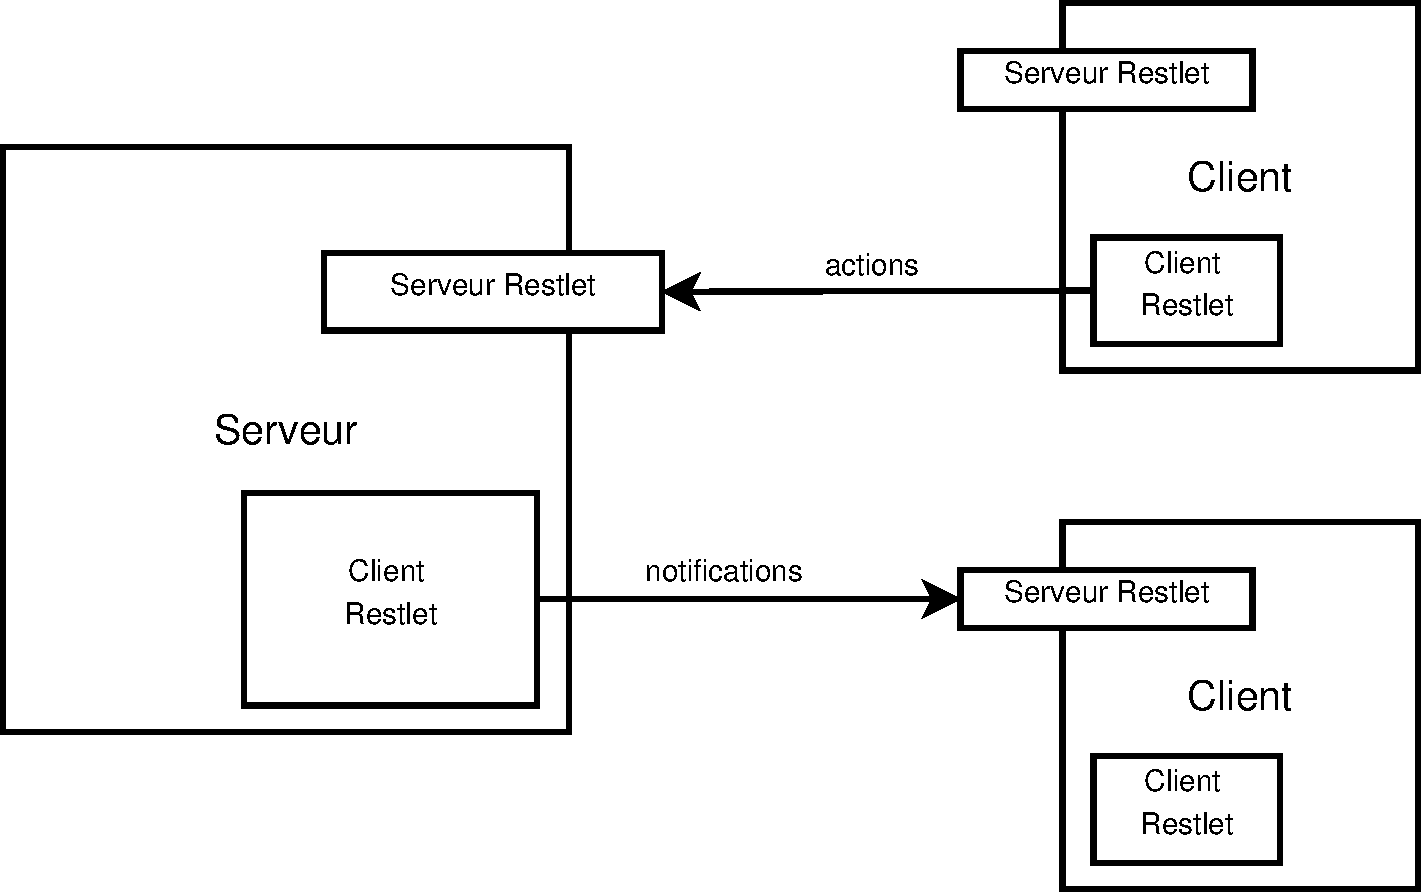
\includegraphics[width=0.8\textwidth]{images/communication}
			\end{center}
			\caption{Principe de communication en entre les clients et le serveur}
			\label{fig:comm}
		\end{figure}
	\end{center}
\end{frame}
